\chapter{Theoretical Background}
\section{Description of generative model}

\subsection{Quantum Circuit Born Machine}
Quantum Circuit Born machines are unsupervised generative models that aim to learn and represent the probability distributions of the dataset through pure quantum states. Through a circuit, we build a parametric ansatz $\psi_{\theta}$, whose wavefunction represents the candidate probability distribution. We will call $D = \{x\}$ our sample dataset, and $\pi$ the target distribution. We measure the projector on the computational base to get the trained probability distribution (through bitstring statistics).
\[ p_{\boldsymbol{\theta}}(x)=\left|\left\langle x \mid \psi_{\boldsymbol{\theta}}\right\rangle\right|^2\]
The objective is to align the model probability distribution $p_{\boldsymbol{\theta}}$ with the target distribution $\pi$.

\subsection{Tensor-Network Born Machine}
Building on the connection between quantum circuits and tensor networks, the canonical form of a Matrix Product State (MPS) provides a simple and natural framework for constructing generative models analogous to Quantum Circuit Born Machines. This correspondence arises from the fact that isometric tensors in an MPS can be mapped to unitary operations in a quantum circuit. Specifically, the virtual bonds of the MPS, which have dimension $D$, can be interpreted as collections of $q$ qubits, where $D=2q$. The isometric tensors are then viewed as columns of a block unitary matrix with a fixed output qubit, assuming a local dimension $d=2$. This mapping allows the MPS to be expressed through a block unitary circuit, where each block unitary is a matrix of size $dD\times dD$. We can generalized this framework to other tensor network architectures such as the Tree Tensor Network (TTN) and the Projected Entangled Pair State (PEPS) \cite{haghshenas_variational_2022}. \\

By leveraging this structural analogy, Tensor-Network Born Machines offer an alternative approach to generative modeling, rooted in the well-established tensor network formalism. In this representation every entry in the tensors composing the network is a possible parameter to be optimized. This "global" approach allows for the design of more expressive models. \\

We can divide training strategies in two main categories: local and global optimization. In a local optimization each tensor, or couple of tensors, is optimized independently, through a sweeping process that iterates over the network, similarly as in DMRG \cite{han_unsupervised_2018} \cite{schollwock_density-matrix_2011}. In a global optimization, all the parameters are optimized simultaneously.

\section{Explicit and Implicit Loss Functions}

An important yet subtle distinction in generative modeling is between explicit and implicit models \cite{rudolph_trainability_2024}. Explicit generative models allow for efficient access to the model probability distribution \( Q_\theta(x) \) for any data sample \( x \). Here, "efficient" means that the probability values can be computed in polynomial time and memory with respect to the size of the data. Once both model's and dataset's probability distributions are knows, a likelihood-based objective function is optimized. A common choice is the minimization of the Kullback-Leibler (KL) divergence:
\[
D_{KL}(P \| Q) = \sum_x P(x) \log \frac{P(x)}{Q_\theta(x)},
\]
where \( P(x) \) is the target distribution, and \( Q_\theta(x) \) is the model's distribution parameterized by \( \theta \).\\
In contrast, implicit generative models do not provide direct access to \( Q_\theta(x) \) but instead allow for efficient sampling from the model distribution. Training is done by comparing the model's samples to the data distribution through a distance measure.
One widely used statistical measure for training implicit models is the Maximum Mean Discrepancy (MMD), which quantifies the difference between two distributions based on their embeddings in a reproducing kernel Hilbert space (RKHS). The MMD is defined as:
\[
\text{MMD}(P, Q_\theta) = \mathbb{E}_{x, x' \sim P}[k(x, x')] - 2\mathbb{E}_{x \sim P, y \sim Q_\theta}[k(x, y)] + \mathbb{E}_{y, y' \sim Q_\theta}[k(y, y')],
\]
where \( k(x, y) \) is a positive-definite kernel function. \\
A prominent example of an implicit generative model is Generative Adversarial Networks (GANs), whose training makes use of the samples produced by the generator to foul the discriminator.
Quantum Circuit Born Machines, when implemented on quantum device, cannot grant explicit access to \( Q_\theta(x) \) but only to samples drawn from the model distribution, measuring the final state of the circuit.

\subsection{Focus on Maximum Mean Discrepancy}

To train the QCBM, we use the squared maximum mean discrepancy (MMD) as the loss function.
\[ 
\mathcal{L}(\boldsymbol{\theta})=\left\|\sum_x p_{\boldsymbol{\theta}}(x) \phi(x)-\sum_x \pi(x) \phi(x)\right\|^2 
\]
where $\phi(x)$ maps $x$ to a larger feature space. Using a kernel $K(x, y)=\phi(x)^T \phi(y)$ allows us to work in a lower-dimensional space. We use the Radial basis function (RBF) kernel for this purpose, which is defined as:
$$
K(x, y)=\frac{1}{c} \sum_{i=1}^c \exp \left(\frac{|x-y|^2}{2 \sigma_i^2}\right)
$$
Here, $\sigma_i$ is the bandwidth parameter controlling the width of the Gaussian kernel. $\mathcal{L}$ approaches to zero if and only if $p_{\boldsymbol{\theta}}$ approaches $\pi$.
We can now write the loss function in terms of $K(x, y)$ as
$$ 
\mathcal{L}=\underset{x, y \sim p_\theta}{\mathbb{E}}[K(x, y)]-2 \underset{x \sim p_\theta, y \sim \pi}{\mathbb{E}}[K(x, y)]+\underset{x, y \sim \pi}{\mathbb{E}}[K(x, y)] 
$$
For discrete distributions, where $p$ and $q$ are represented as vectors (or histograms) and the kernel matrix $K$ is computed over a discrete “space” [1], [2], the above expression reduces to:
$$ 
\left(p_x-p_y\right)^{\top} K\left(p_x-p_y\right) 
$$
This is the expression used to calculate MMD in case of a QCBM, and involves summing over the set of all possible bitstrings that the model can generate, an exponential number of terms. This is computationally infeasible for large systems. In our "dequantized" tensor network representation we wanto to find a way to calculate the MMD loss function efficiently, leveraging tensor network contractions.

\section[Efficient loss calculation with tensor network]{Efficient loss calculation with tensor network}
The Maximum Mean Discrepancy (MMD) is a distance measure between two probability distributions based on the expectation values of a positive semi-definite kernel function $ K(x, y) $. In our context, it is used to compare the distribution $ q_\theta(x) $, generated by a quantum model, with a target distribution $ p(x) $ obtained from classical data. The data samples $ y $ are bitstrings, i.e., elements of the computational basis.

\begin{equation}
\operatorname{MMD}(\theta) = 
\sum_{x \in \Omega} \sum_{y \in \Omega} q_{\theta}(x) K(x, y) q_{\theta}(y)
+ \sum_{x \in T} \sum_{y \in T} p(x) p(y) K(x, y)
- 2 \sum_{x \in \Omega} \sum_{y \in T} q_\theta(x) K(x, y) p(y),
\end{equation}
where the Born rule is applied as $ q_\theta(x) = |\braket{x | \psi}|^2 $.
The optimization problem can then be expressed as:
\begin{equation}
\min_{\theta} \operatorname{MMD}(\theta) =
\min_{\theta} \bigg[ 
\sum_{x, y \in \Omega} |\braket{x | \psi}|^2 K(x, y) |\braket{y | \psi}|^2
- 2 \sum_{x \in \Omega} \sum_{y \in T} |\braket{x | \psi}|^2 K(x, y) p(y) 
\bigg].
\end{equation}

We can manually contruct the TN that represents the sampling probabilities of the state $\ket{\psi}$. For example, for a single biststring $b = b_1\ldots b_n$, the probability of sampling it is given by

$$p(b) = |\langle\psi|\bm{b}\rangle|^2 = \langle\psi|b\rangle \langle b|\psi\rangle = \langle\psi|\Pi_{b}|\psi\rangle$$

where in the last equation we defined the projector $\Pi_b = |b\rangle\langle b|$ corresponding to bitstring $b$. Now, focus on a single qubit and imagine we put together in a list the projectors on state $\ket{0}$ and $\ket{1}$, thus obtaining

$$\Pi = [\Pi_0, \Pi_1], \quad \Pi_0 = |0\rangle\langle0|, \Pi_1 = |1\rangle\langle1|$$

This object $\Pi$ is a tensor of dimensions (2, 2, 2), and it is essentially a representation of the POVM corresponding to measuring in the computational basis $Z$. One can then construct a TN that encodes the sampling probabilities from state $\ket{\psi}$ by using the formula above 

$$p(b_1b_2\ldots b_n) = \langle\psi|\Pi_{b_1} \otimes \Pi_{b_2} \ldots \otimes \Pi_{b_n}|\psi\rangle$$

where each of the local $\Pi_b$ is the (2,2,2) tensors introduced above. Imporantly, this is a tensor networks where the open legs are the outcomes one $b_i$.
For a single-qubit space, measuring only in $Z$ basis, this corresponds to 
$$
\left[
\begin{array}{cc|cc}
1 & 0 & 0 & 0 \\
0 & 0 & 0 & 1
\end{array}
\right]
$$

For each node of the tensor network. We can create the single node and put them together in an MPO

The expression $ \, p(b_1b_2\ldots b_n) = \langle\psi|\Pi_{b_1} \otimes \Pi_{b_2} \ldots \otimes \Pi_{b_n}|\psi\rangle \,$
can be built as:
\begin{figure}[h]
    \centering
    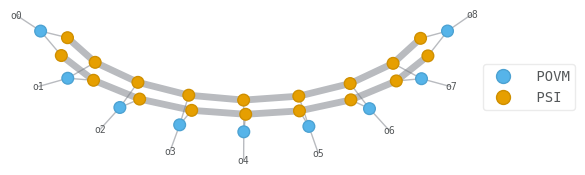
\includegraphics[width=0.8\textwidth]{images/new/probs_tn.png}
    \caption{Tensor network representation of the sampling probabilities $p(b_1b_2\ldots b_n)$. Each node corresponds to a local projector $\Pi_{b_i}$, and the open legs represent the outcomes $b_i$.}
    \label{fig:probs_tn}
\end{figure}

The expression above become:

$$
= \min \left[
\sum_{x, y} \braket{\psi | \Pi | \psi} K(x, y) \braket{\psi | \Pi | \psi}
- 2 \sum_{x} \sum_{y} \braket{\psi | \Pi | \psi} K(x, y) p(y)
\right]
$$
\\
The kernel matrix $ K $ is defined as
$$
K = 
\begin{pmatrix}
1 & e^{-\frac{1}{2\sigma^2}} \\
e^{-\frac{1}{2\sigma^2}} & 1
\end{pmatrix}
$$\\
which encodes similarity between bitstrings using a Gaussian function. This matrix acts on the output space indexed by $ x $ and $ y $, and can be realized as a kernel MPO.\\
In full tensor index notation, the MMD becomes:

$$
\begin{aligned}
= \psi_b \, \Pi_k^{b, o} \, \psi^k \, K_{o}^{o'} \, \psi_b \, \Pi_k^{b, o'} \, \psi^k 
- 2\,\sum_B \left[ 
\psi^b \, \Pi_b^{ko} \, \psi_k \, K_{o}^{o'} \, B^o
\right]
\end{aligned}
$$

Here, $ \psi^k $ and $ \psi_b $ are the components of the quantum state $ \ket{\psi} $ and its dual $ \bra{\psi} $, respectively. Indices are placed according to the usual tensor convention: kets carry upper indices and bras lower indices. The operator $ \Pi $ is a tensor with indices $ \Pi_k^{b, o} $, encoding its action on both input and measurement bases. The sum over $ B $ denotes averaging over the target data bitstrings $ y $, with $ B^o $ representing the empirical frequency vector from data.

The first term can be built as:
\begin{figure}[h]
    \centering
    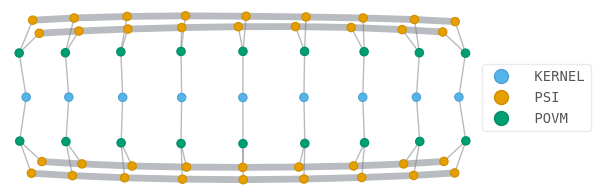
\includegraphics[width=0.8\textwidth]{images/new/overlap_tn.png}
    \caption{Tensor network representation of the first term in the MMD expression. The kernel matrix $ K $ acts on the output space indexed by $ x $ and $ y $, and can be realized as a kernel MPO.}
    \label{fig:overlap_tn}
\end{figure}\\
The second term needs the MPS representation of data. We are going to build a "computational MPS" for each bitstring in the dataset, which can be thought as the eigenstate that gives every time we sample the original bitstring. To compute efficiently the sum over the all possible bitstrings, we can group all the computational MPS in an hyperindexed tensor network, quimb will then sum over the hyperindex efficently.
\begin{figure}[h]
    \centering
    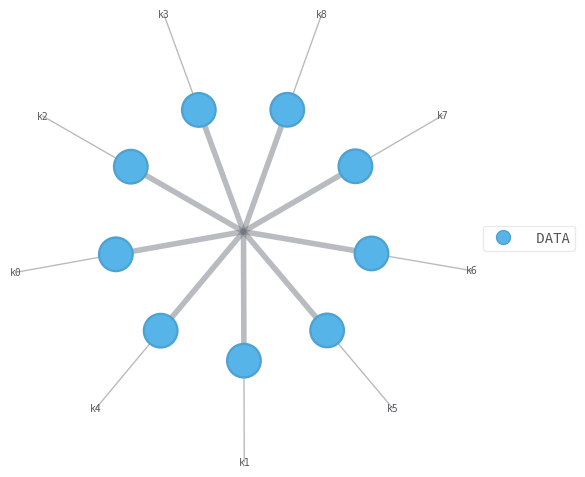
\includegraphics[width=0.5\textwidth]{images/new/data_tn.png}
    \caption{The data bitstrings are represented as computational MPS, and the hyperindex allows efficient summation over all possible bitstrings.}
    \label{fig:data_tn}
\end{figure}\\
The mixed term of the MMD can be built as:
\begin{figure}[h]
    \centering
    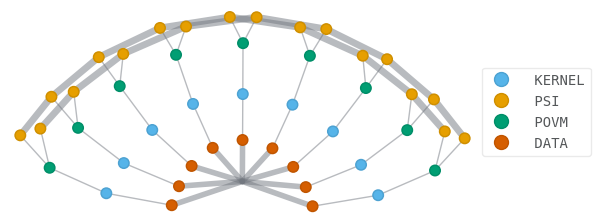
\includegraphics[width=0.5\textwidth]{images/new/overlap_data_tn.png}
    \caption{Tensor network representation of the mixed term in the MMD expression. The kernel matrix $ K $ acts on the output space indexed by $ x $ and $ y $, and can be realized as a kernel MPO.}
    \label{fig:overlap_data_tn}
\end{figure}\\

\subsection{Appendix: other measures}

\subsubsection{MMD as MPO as sum of operators of different bodyness}

Let's consider the MMD loss function defined as:
$$  
\mathcal{L}_{\mathrm{MMD}}(\boldsymbol{\theta})=\underset{x, y \sim p_\theta}{\mathbb{E}}[K(x, y)]-2 \underset{x \sim p_\theta, y \sim \pi}{\mathbb{E}}[K(x, y)]+\underset{x, y \sim \pi}{\mathbb{E}}[K(x, y)] =\sum_{\boldsymbol{x}, \boldsymbol{y} \in \mathcal{X}} q_{\boldsymbol{\theta}}(\boldsymbol{x}) q_{\boldsymbol{\theta}}(\boldsymbol{y}) K(\boldsymbol{x}, \boldsymbol{y})-2 \sum_{\boldsymbol{x}, \boldsymbol{y} \in \mathcal{X}} q_{\boldsymbol{\theta}}(\boldsymbol{x}) p(\boldsymbol{y}) K(\boldsymbol{x}, \boldsymbol{y})+\sum_{\boldsymbol{x}, \boldsymbol{y} \in \mathcal{X}} p(\boldsymbol{x}) p(\boldsymbol{y}) K(\boldsymbol{x}, \boldsymbol{y}) 
$$

where

$$ 
\begin{aligned} K_\sigma(\boldsymbol{x}, \boldsymbol{y}) =e^{-\frac{\|\boldsymbol{x}-\boldsymbol{y}\|_2^2}{2 \sigma}}  =\prod_{i=1}^n e^{-\frac{\left(x_i-y_i\right)^2}{2 \sigma}},\end{aligned}
$$
We can rewrite each term in MMD loss as an expectation value of an observable:
$$ \mathcal{M}\left(\rho, \rho^{\prime}\right)=\operatorname{Tr}\left[O_{\mathrm{MMD}}^{(\sigma)}\left(\rho \otimes \rho^{\prime}\right)\right] $$
where
$$
O_{\mathrm{MMD}}^{(\sigma)}:=\sum_{\boldsymbol{x}, \boldsymbol{y}} K_\sigma(\boldsymbol{x}, \boldsymbol{y})|\boldsymbol{x}\rangle\langle\boldsymbol{x}| \otimes|\boldsymbol{y}\rangle\langle\boldsymbol{y}|
$$
We can also rewrite the observable as the sum of Puli strings, each one containing
$$
O_{\mathrm{MMD}}^{(\sigma)}=\sum_{l=0}^n\binom{n}{l}\left(1-p_\sigma\right)^{n-l} p_\sigma^l D_{2 l}
$$
where
$$ D_{2 l}=\frac{1}{\binom{n}{l}} \sum_{\substack{A \subseteq \mathcal{N} \\|A|=l}} \bigotimes_{i \in A}\left(Z_i \otimes Z_{n+i}\right) $$
where the summation runs over all possible combinations of strings of length l
$ A \subseteq \mathcal{N}=\{1,2, \ldots, n\} $
and
$ p_\sigma=\left(1-e^{-1 /(2 \sigma)}\right) / 2 $.
\begin{figure}[h]
    \centering
    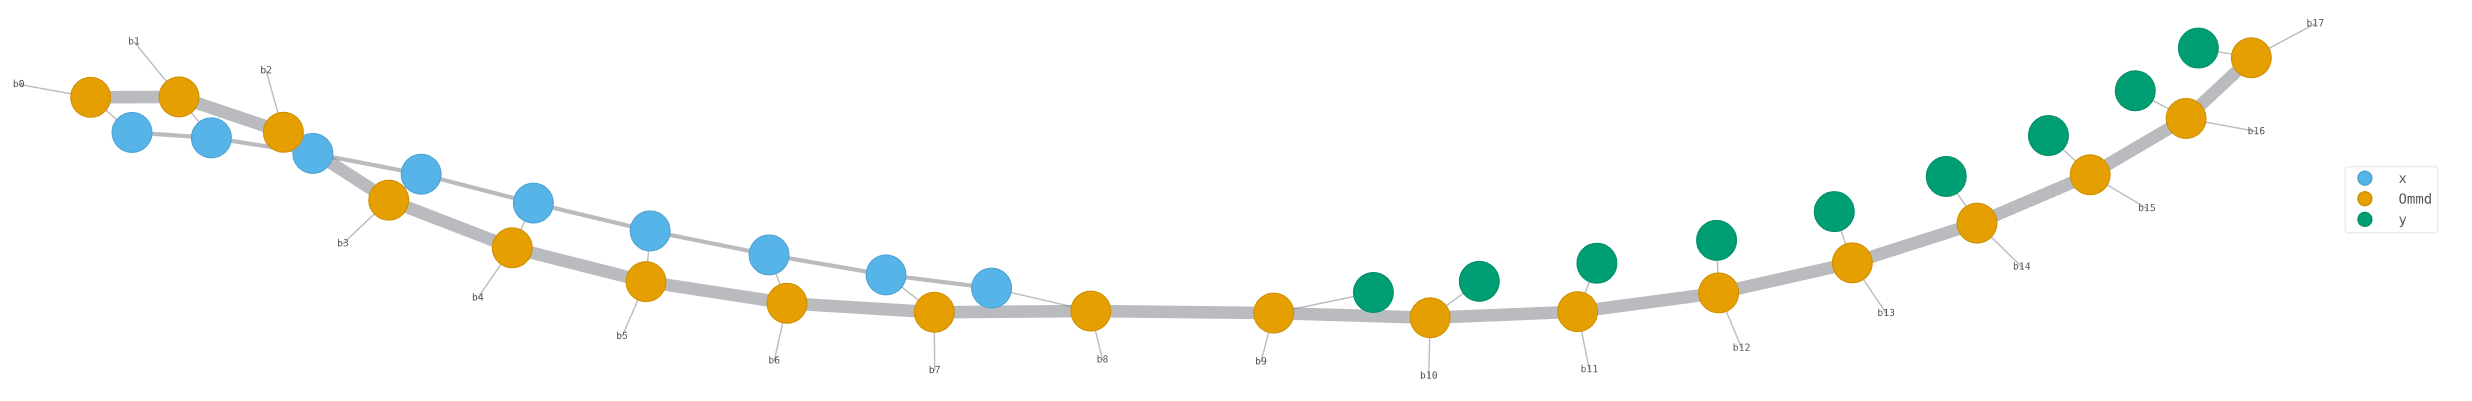
\includegraphics[width=0.5\textwidth]{images/mpo1.png}
    \caption{We contract the model (in blue) and the data (green) with the MPO representing the loss function (organge). - figure to bi fixed, I didn't noticed the legend was not rendered}
    \label{fig:example}
\end{figure}

\subsubsection{Local quantum fidelity}
$L_{a F}^{(e)}=1-\left\langle N_O\right| H_L|\varphi\rangle$, where $H_L=\left.\frac{1}{m} \sum_{i=1}^m|0\rangle\langle 0| \otimes 1\right|_{\bar{i}}$, whare $\bar{i}$ undicale all qubits except $i=$
$$
\begin{aligned}
=\frac{1}{m}\left[\left(\begin{array}{c}
|0\rangle\langle 0| \\
\mathbb{I}  \\
\mathbb{I}  \\
\vdots
\end{array}\right)+\left(\begin{array}{c}
\mathbb{I} \\
|0\rangle\langle 0| \\
\mathbb{I}  \\
\mathbb{I}  \\
\vdots
\end{array}\right)+\ldots+\left(\begin{array}{c}
\mathbb{I} \\
\mathbb{I} \\
\cdots \\
\\
|0\rangle\langle 0|
\end{array}\right)\right]=
\end{aligned}
$$
\[
\left[
\begin{array}{c}
\left(\begin{array}{cc}
1 & 0 \\
0 & \frac{n-1}{m}
\end{array}\right) \\[10pt]
\left(\begin{array}{cc}
1 & 0 \\
0 & \frac{n-1}{m}
\end{array}\right) \\[10pt]
\vdots
\end{array}
\right] = MPO
\]


